% BEGIN PREAMBEL
\documentclass[9pt]{beamer}
\usepackage[british]{babel}
\usepackage[latin1]{inputenc}
\usepackage{amsmath,amsfonts,amssymb}
\usepackage{upgreek}
\usepackage{pgfpages}
\usepackage[version=3]{mhchem}
\usepackage{lmodern}
\usepackage{graphicx}
\usepackage{multicol}
\usepackage{xcolor}
\usepackage{wrapfig}
\newcommand{\as}{\\[14pt]}
\newcommand{\s}{\\[7pt]}
\newcommand{\is}{\\[2pt]}
\newcommand{\no}{\noindent}
\newcommand{\ka}{\hspace*{0.5cm}}
\newcommand{\ma}{\hspace*{1cm}}
\newcommand{\ga}{\hspace*{1.5cm}}
\newcommand{\li}{\left|}
\newcommand{\re}{\right|}
\newcommand{\const}{\text{const.}}
\newcommand{\z}{\text}
\newcommand{\terminal}[1]{\colorbox{black}{\textcolor{white}{{\fontfamily{phv}\selectfont \scriptsize{#1}}}}}
\newcommand{\plugin}[1]{\textit{\flq#1\frq}}
\usetheme{Boadilla}
\usecolortheme{beaver}
\useoutertheme{miniframes}
\beamertemplatenavigationsymbolsempty
\makeindex
\title[Analysis]{Discussion of the Pad Analysis}
\author[M. Reichmann]{Michael Reichmann}
\institute[\textbf{\textit{ETH}}\scalebox{.6}{\textit{Z\"{u}rich}}]{Swiss Federal Institute of Technology Zurich}
% END PREAMBEL
\begin{document}
% ============================
% TITLE PAGE
% ============================
\begin{frame}
	\begin{center}
		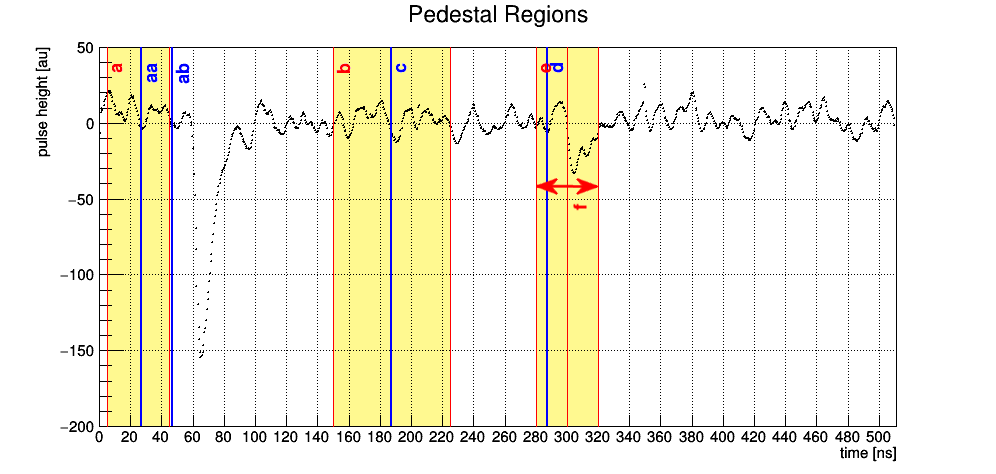
\includegraphics[width=8cm]{Pics/PedestalRegions}
	\end{center}
	\begin{alertblock}{
		\begin{center}
			\textbf{Preliminary Results of Pixel Detectors in 2015 PSI Testbeams}
		\end{center}}
		\vspace*{10pt}
		\begin{center}\small
		Michael Reichmann
		\end{center}\normalsize
	\end{alertblock}
\end{frame}
% ====================================================================================
% TELESCOPE
% ====================================================================================
\section{Regions}
\begin{frame}
	\begin{center}
		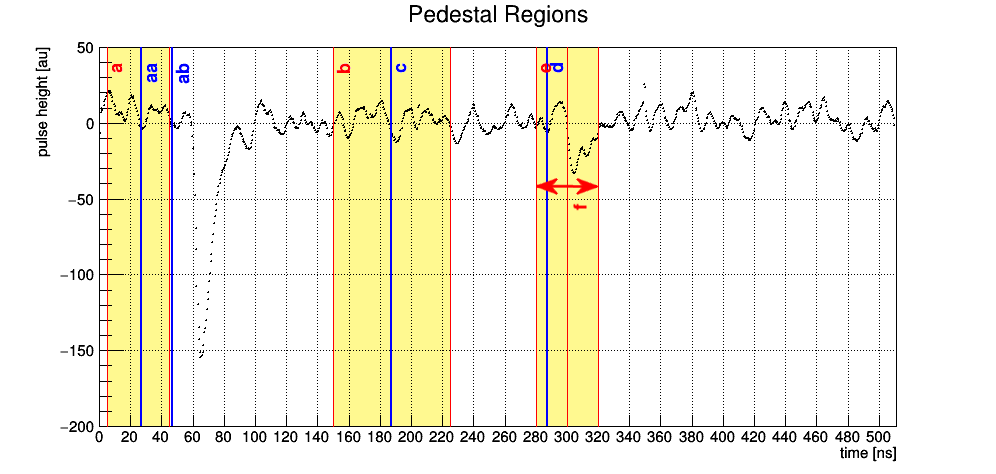
\includegraphics[width=\textwidth]{Pics/PedestalRegions}
	\end{center}
	\begin{itemize}
		\item 
	\end{itemize}
\end{frame}
% new frame ============================
\begin{frame}
	\begin{center}
		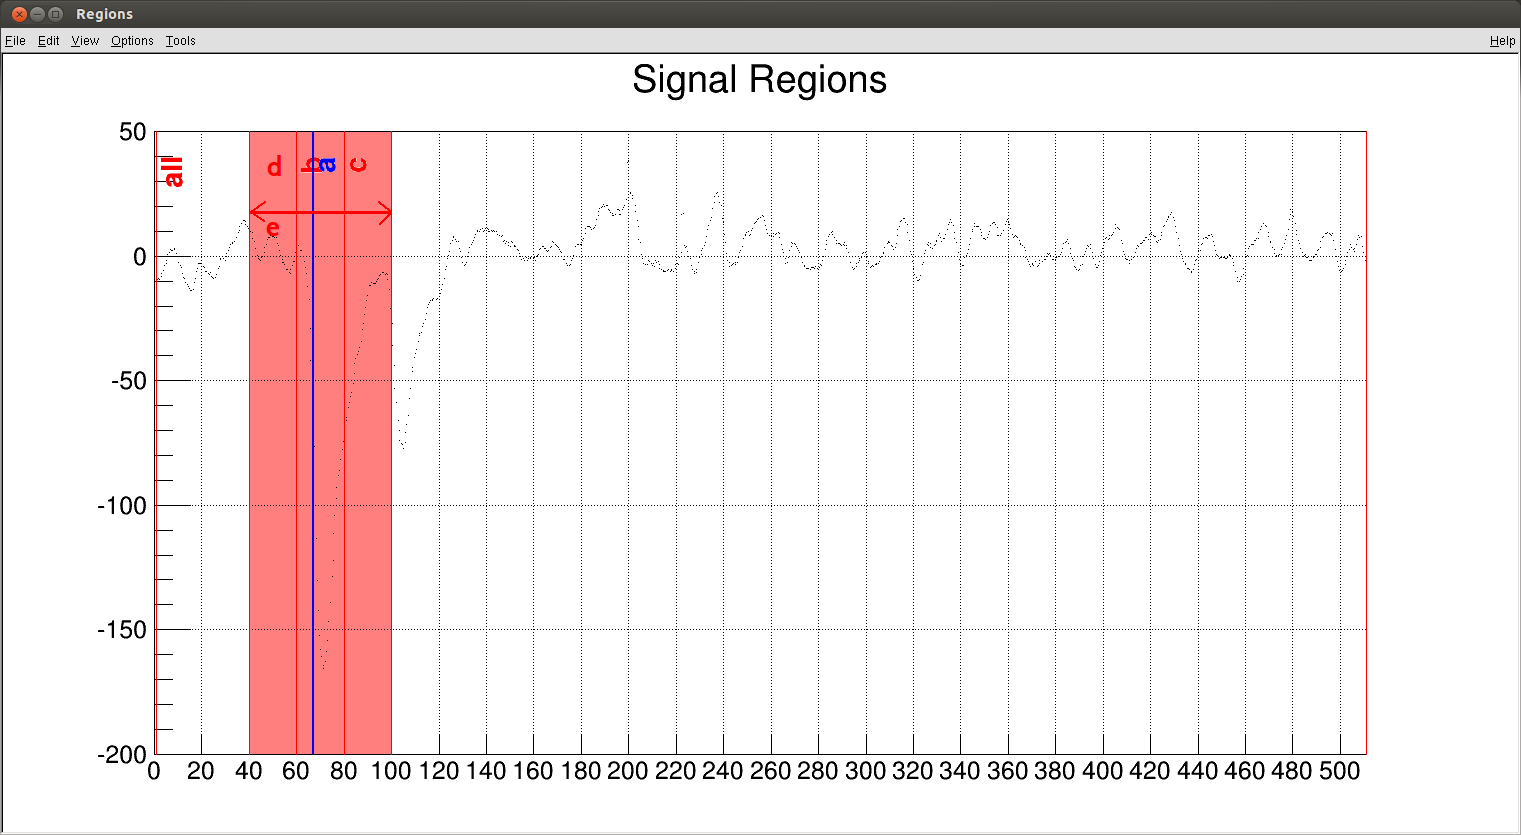
\includegraphics[width=\textwidth]{Pics/SignalRegions}
	\end{center}
	\begin{itemize}
		\item 
	\end{itemize}
\end{frame}
% new frame ============================
\begin{frame}
	\begin{itemize}
		\item Status a the last meeting
	\end{itemize}
	\begin{center}
		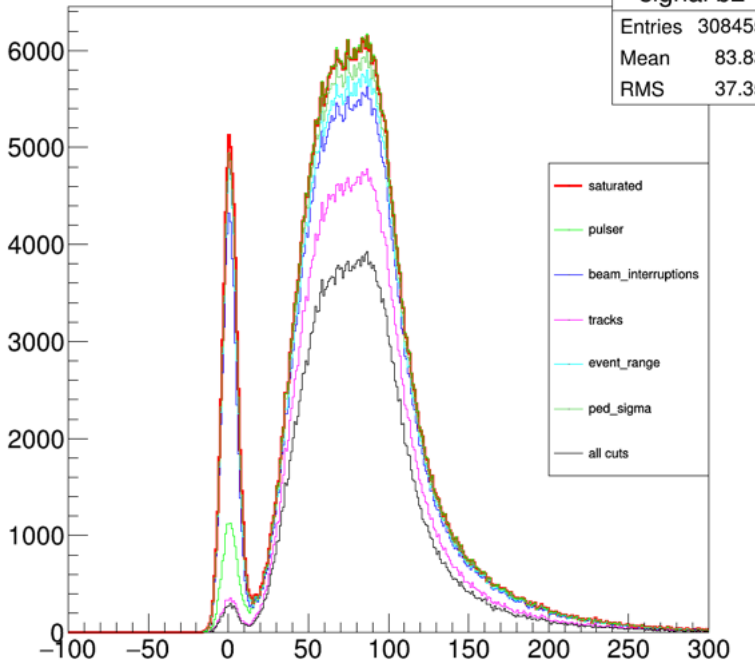
\includegraphics[width=8cm]{Pics/oldcuts}
	\end{center}
\end{frame}
% new frame ============================
\begin{frame}
	\begin{center}
		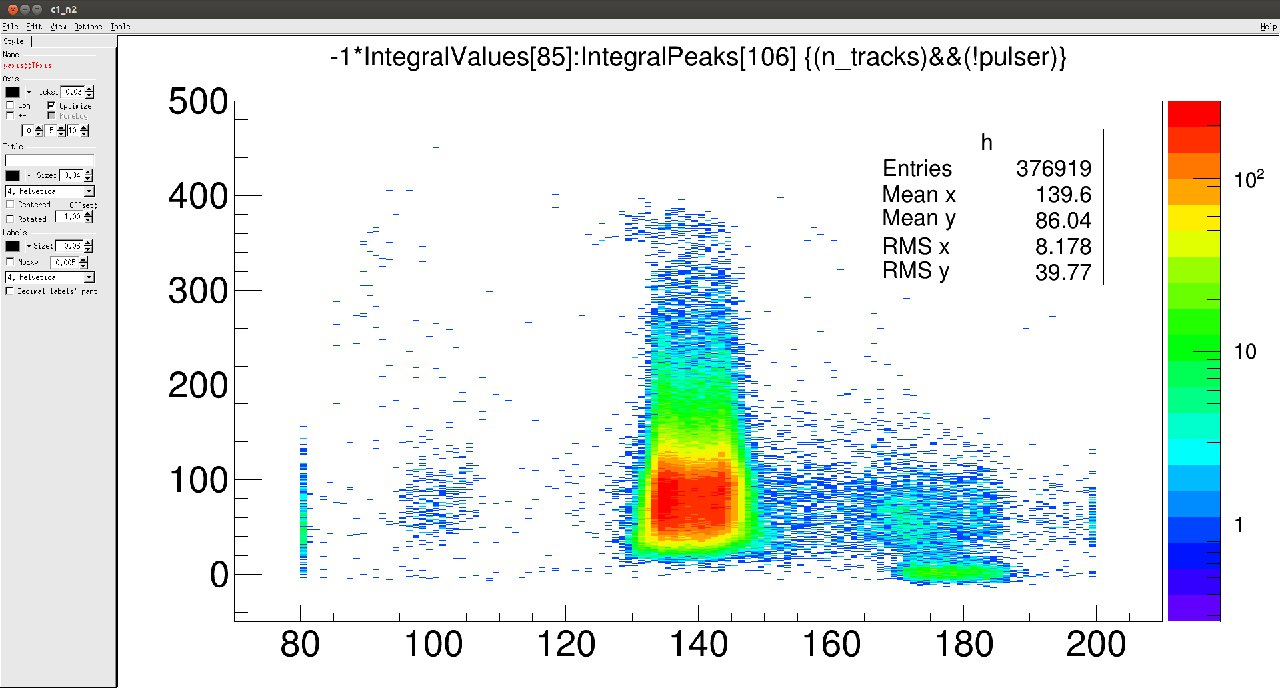
\includegraphics[width=8cm]{Pics/Buckets1}
	\end{center}
	\begin{itemize}
		\item second setup
	\end{itemize}
\end{frame}
% new frame ============================
\begin{frame}
	\begin{center}
		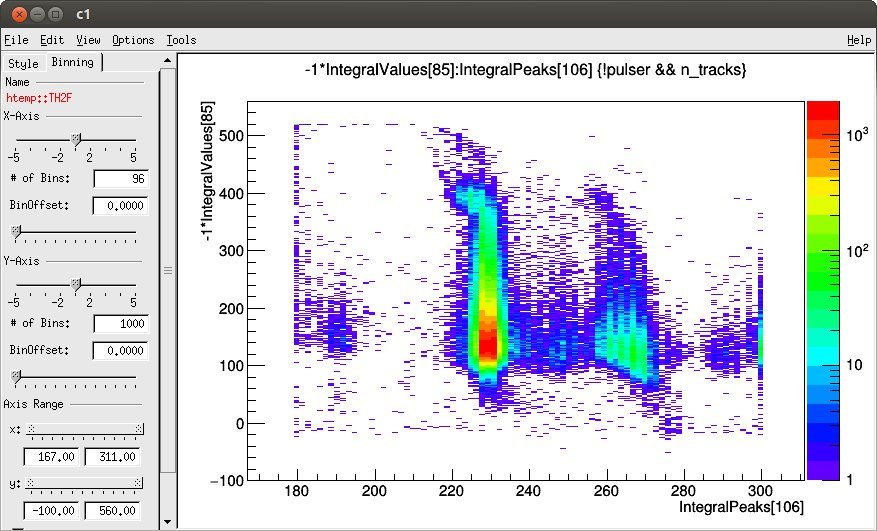
\includegraphics[width=8cm]{Pics/Buckets2}
	\end{center}
	\begin{itemize}
		\item first setup
	\end{itemize}
\end{frame}
% new frame ============================
\begin{frame}
	\begin{center}
		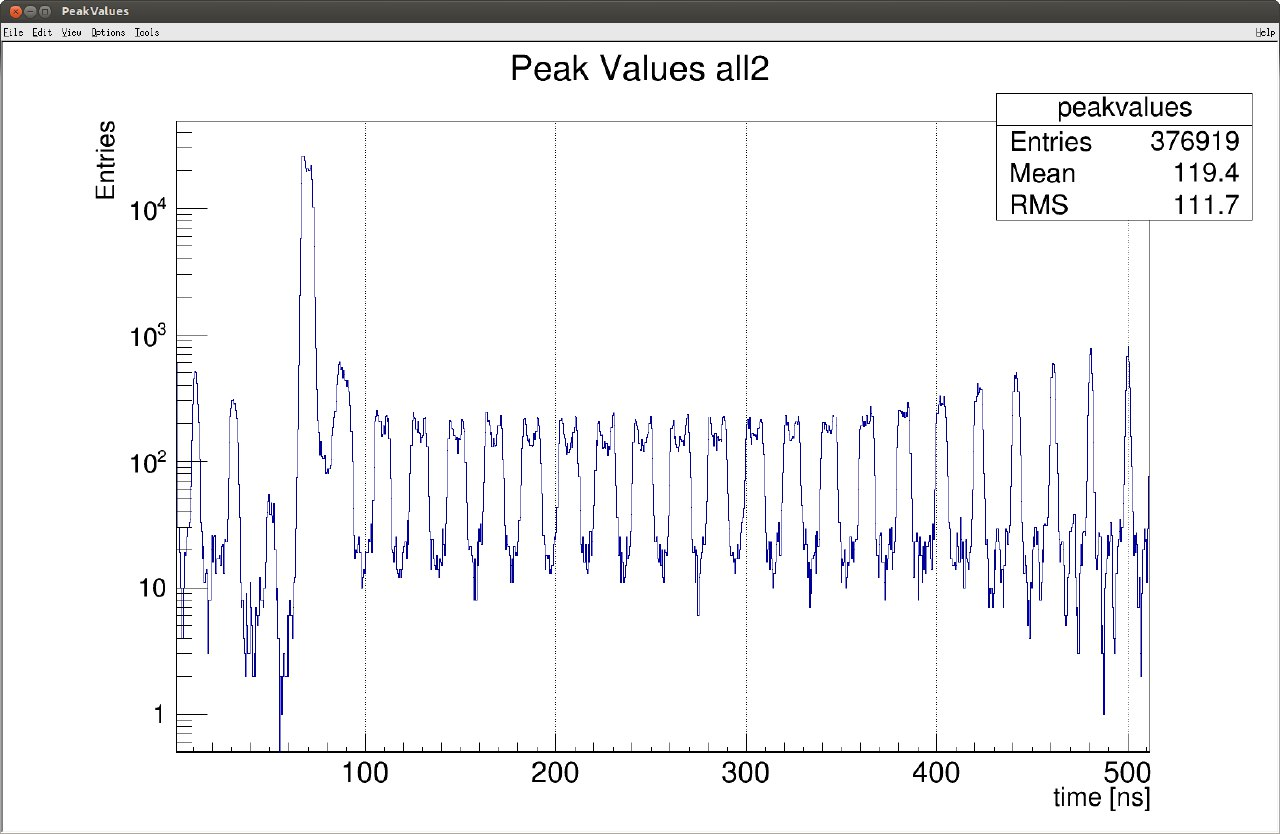
\includegraphics[width=8cm]{Pics/peakvalues}
	\end{center}
	\begin{itemize}
		\item first setup
	\end{itemize}
\end{frame}
% new frame ============================
\begin{frame}
	\frametitle{Additional Cuts}
	\begin{itemize}
		\item chi2
		\begin{itemize}
% 			\item take only tracks with \Upchi$^{2}$ in 90\% Quantile
			\item chi2\_tracks$<$29.499836262\&\&chi2\_tracks$>=$0
		\end{itemize}
		\item track angle
		\begin{itemize}
			\item take only tracks in a certain angle range around the mean angle
			\item slope\_x$>$-2.72731579593\&\&slope\_x$<$1.27268420407\&\&slope\_y$>$-1.6885275642\&\&slope\_y$<$2.3114724358
		\end{itemize}
		\item bucket cut 
		\begin{itemize}
			\item take only events where the max in the signal region is higher than in the buckets in front and after the signal region
			\item $-1*IntegralValues[106]--1*IntegralValues[85]==0$
			\item improve cut: if max in bucket 1 or -1 is larger than in bucket 0, signal in bucket 0 has to be below a threshold (is ped event)
		\end{itemize}
		\item add cut on pad region, landau gets more confined?
	\end{itemize}
\end{frame}
% new frame ============================
\begin{frame}
	\begin{center}
		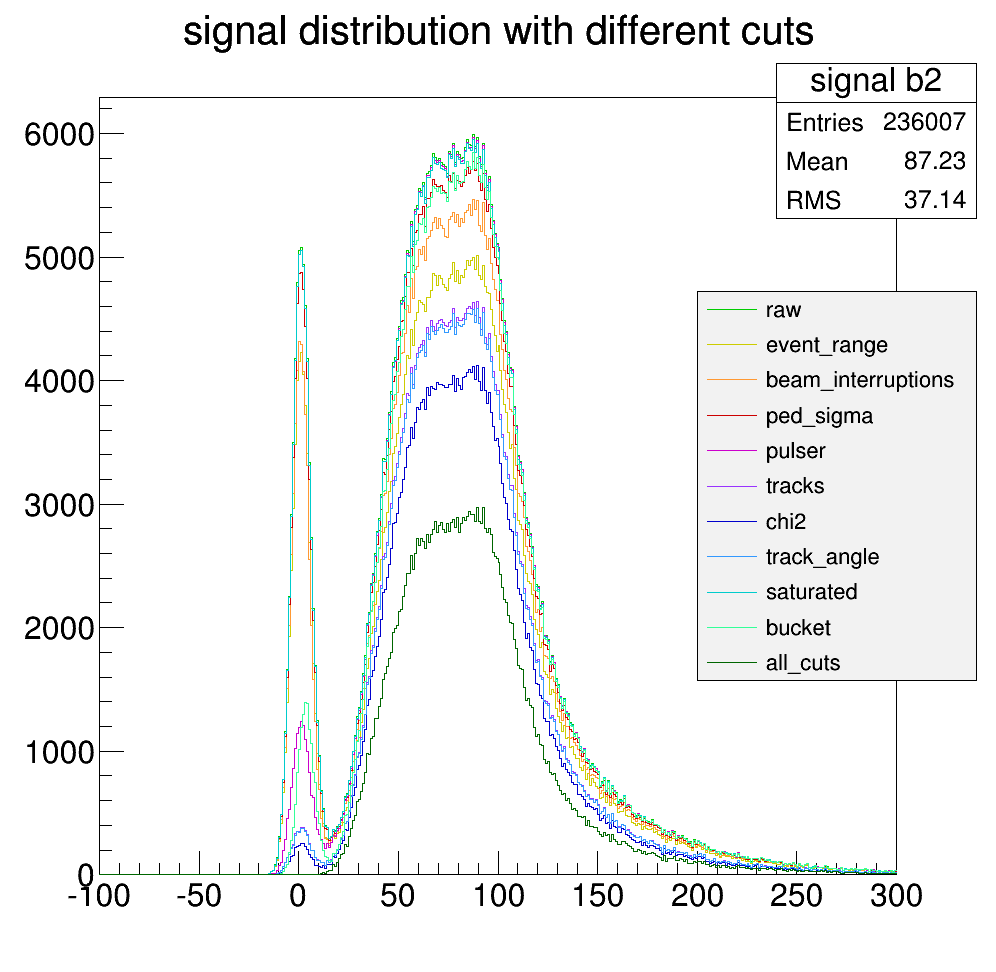
\includegraphics[width=8cm]{Pics/all}
	\end{center}
	\begin{itemize}
		\item 
	\end{itemize}
\end{frame}
% new frame ============================
\begin{frame}
	\begin{center}
		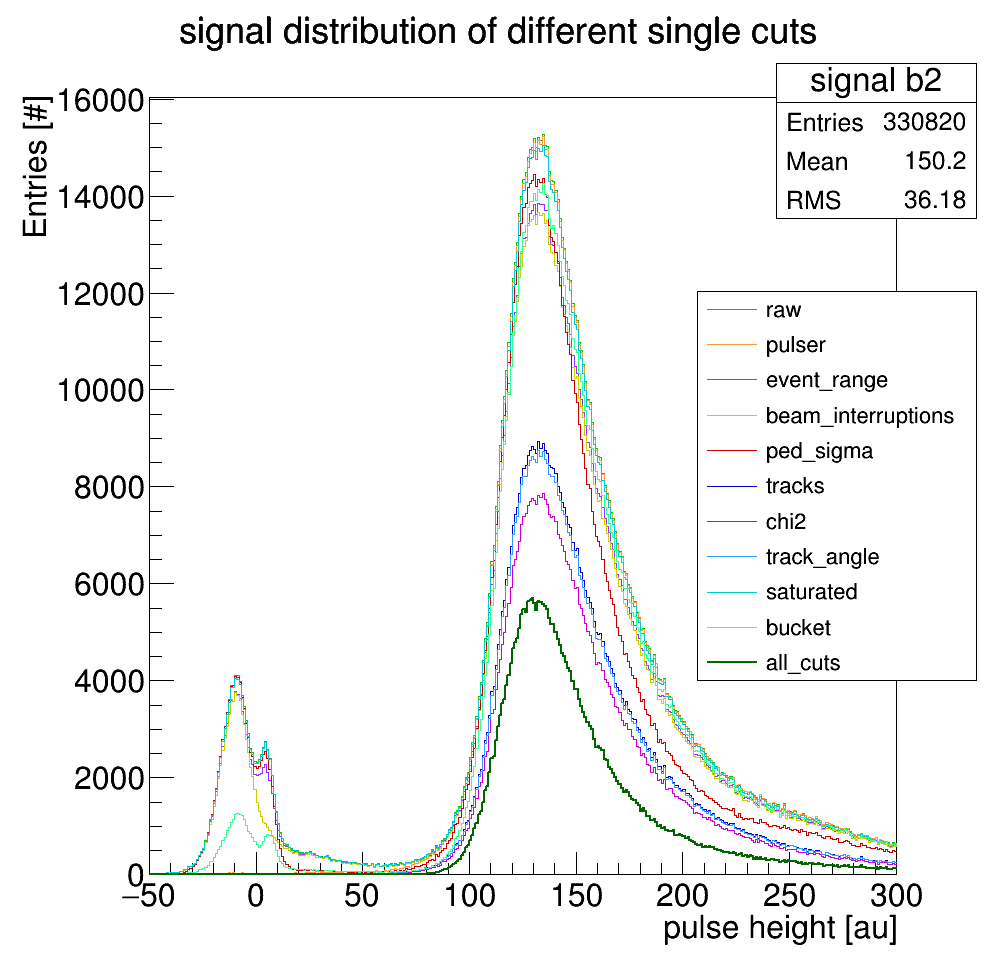
\includegraphics[width=8cm]{Pics/augustcuts}
	\end{center}
	\begin{itemize}
		\item 
	\end{itemize}
\end{frame}
% new frame ============================
\begin{frame}
	\begin{center}
		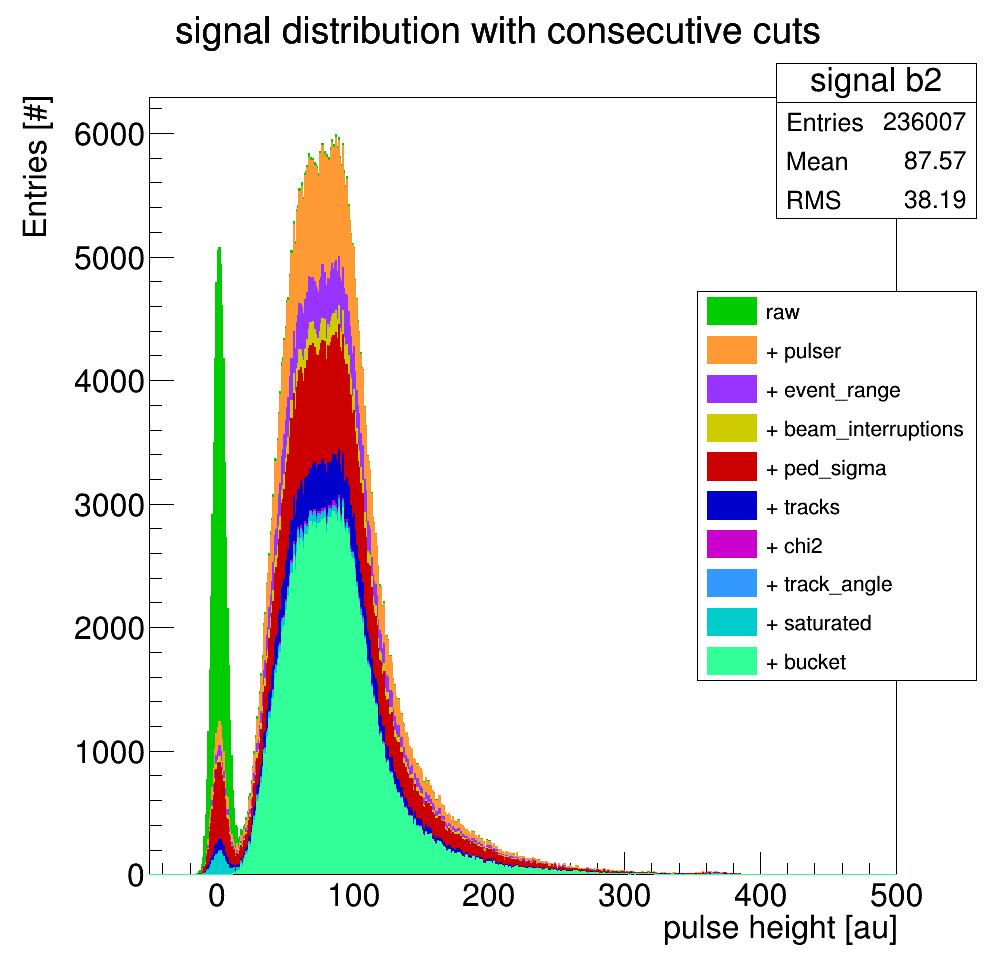
\includegraphics[width=8cm]{Pics/consecutive}
	\end{center}
	\begin{itemize}
		\item 
	\end{itemize}
\end{frame}
% new frame ============================
\begin{frame}
	\begin{center}
		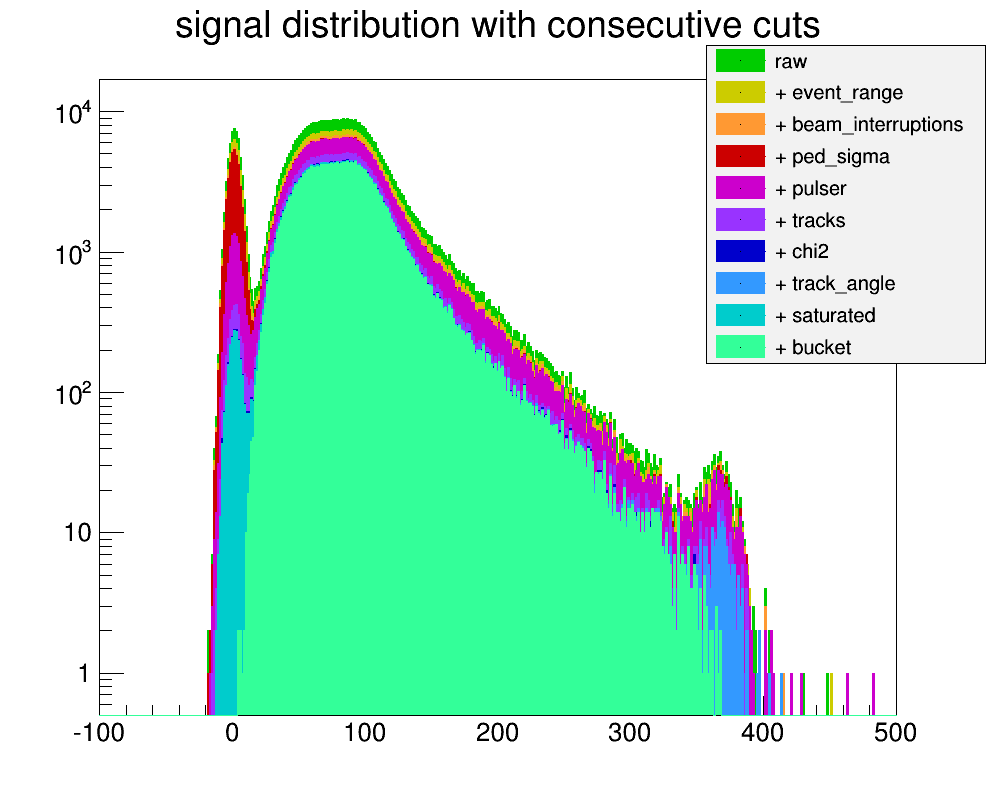
\includegraphics[width=8cm]{Pics/ConsLog}
	\end{center}
	\begin{itemize}
		\item 
	\end{itemize}
\end{frame}
% new frame ============================
\begin{frame}
	\begin{center}
		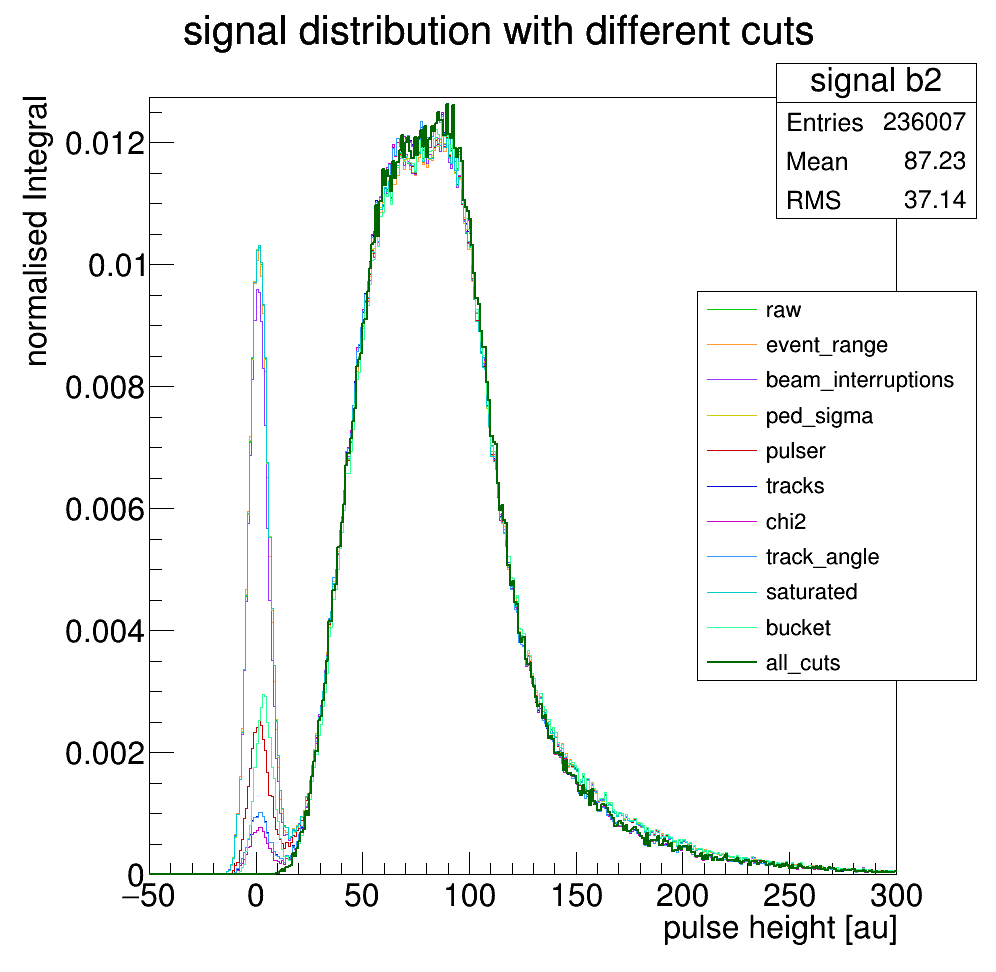
\includegraphics[width=8cm]{Pics/normalised}
	\end{center}
	\begin{itemize}
		\item 
	\end{itemize}
\end{frame}
% new frame ============================
\begin{frame}
	\frametitle{Landau attributes of different cuts}
	\begin{center}
		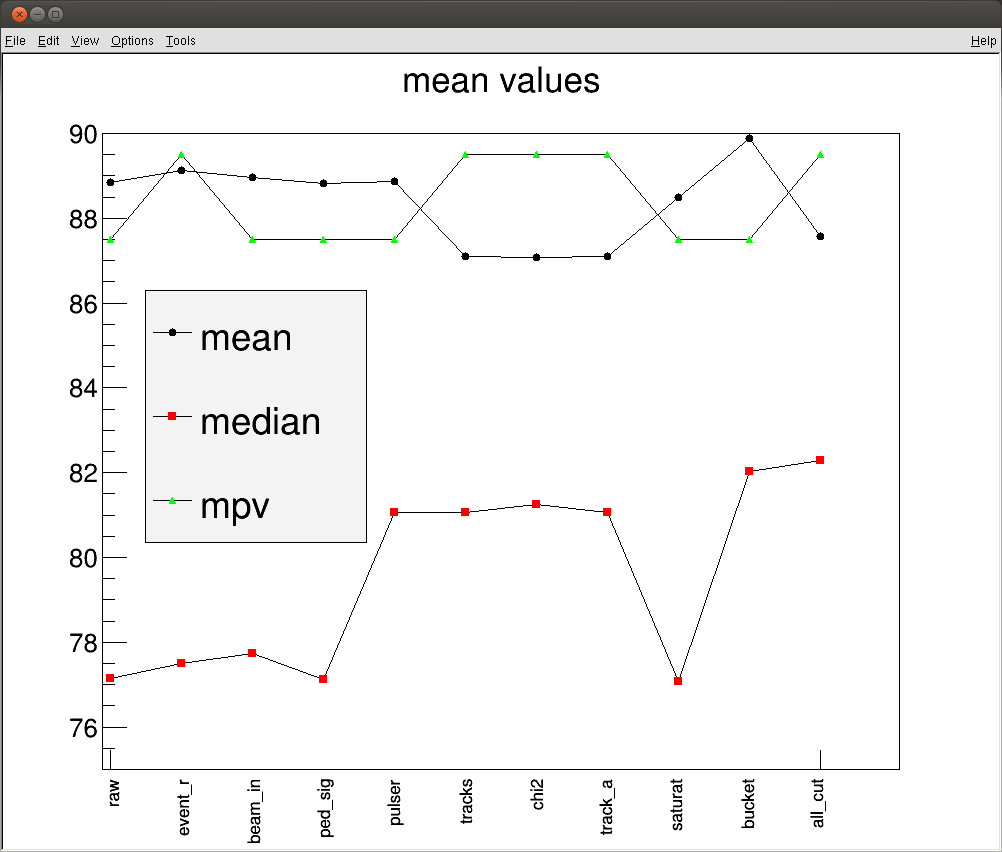
\includegraphics[width=8cm]{Pics/landaucuts}
	\end{center}
	\begin{itemize}
		\item 
	\end{itemize}
\end{frame}
% new frame ============================
\begin{frame}
	\frametitle{Pedestals of Different runs}
	\begin{center}
		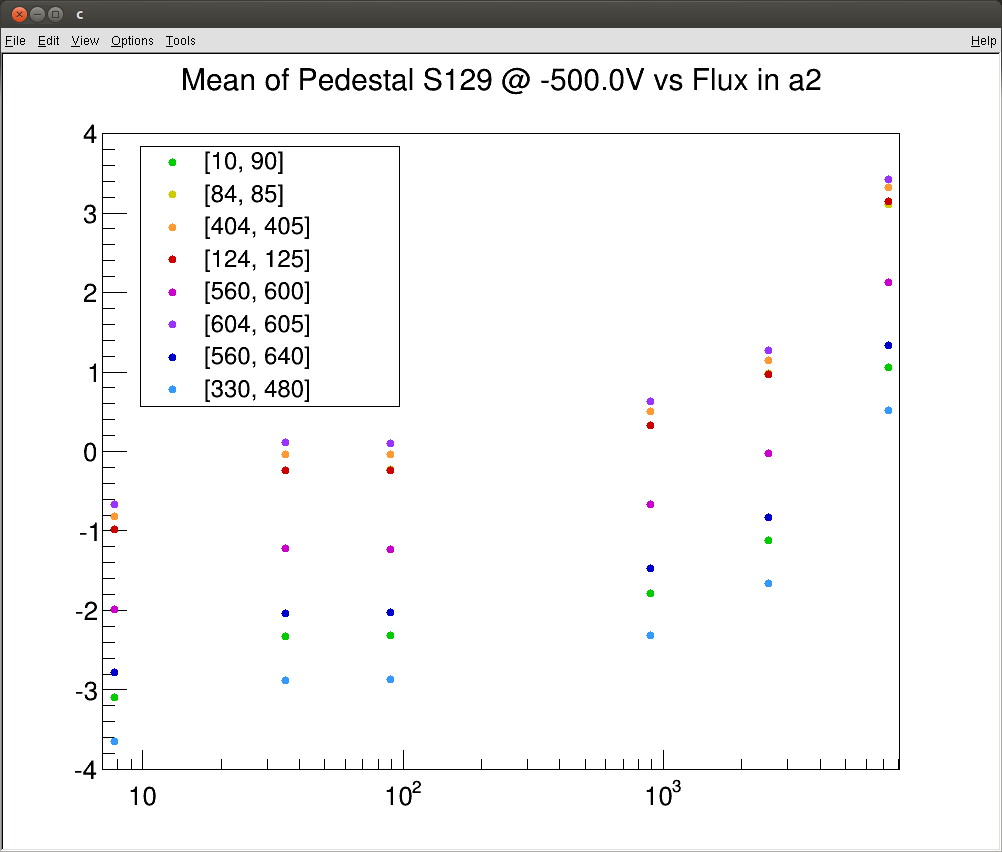
\includegraphics[width=8cm]{Pics/meanPedestals}
	\end{center}
	\begin{itemize}
		\item 
	\end{itemize}
\end{frame}
% new frame ============================
\begin{frame}
	\frametitle{Signal S129}
	\begin{center}
		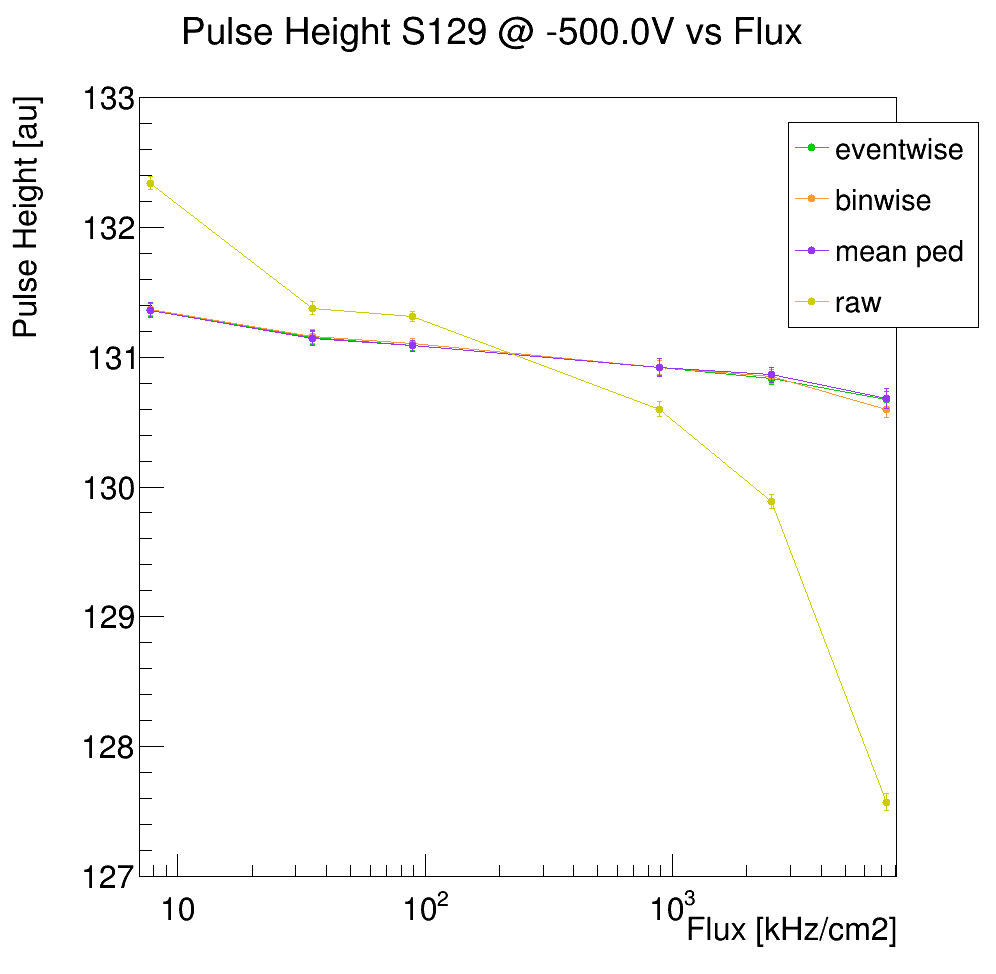
\includegraphics[width=7cm]{Pics/sig129}
	\end{center}
\end{frame}
% new frame ============================
\begin{frame}
	\frametitle{Signal S129}
	\begin{center}
		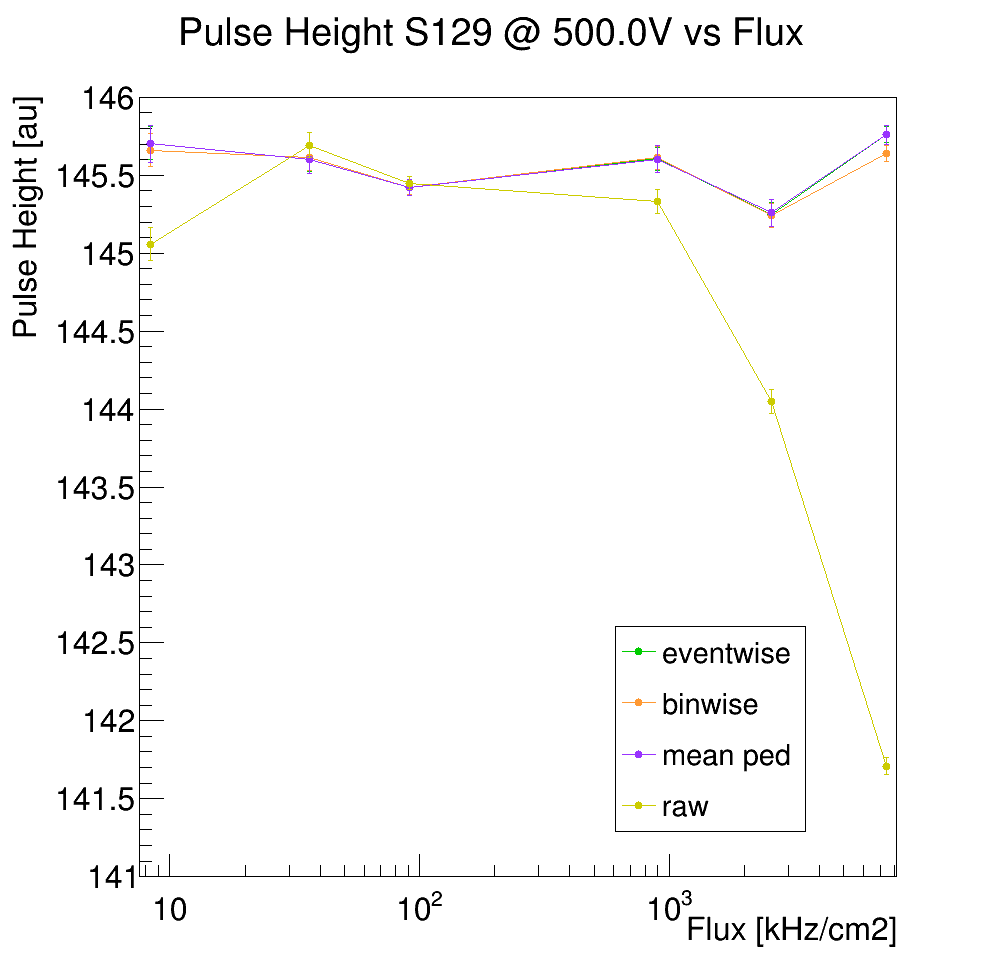
\includegraphics[width=7cm]{Pics/sig129pos}
	\end{center}
\end{frame}
% new frame ============================
\begin{frame}
	\frametitle{Signal B2}
	\begin{center}
		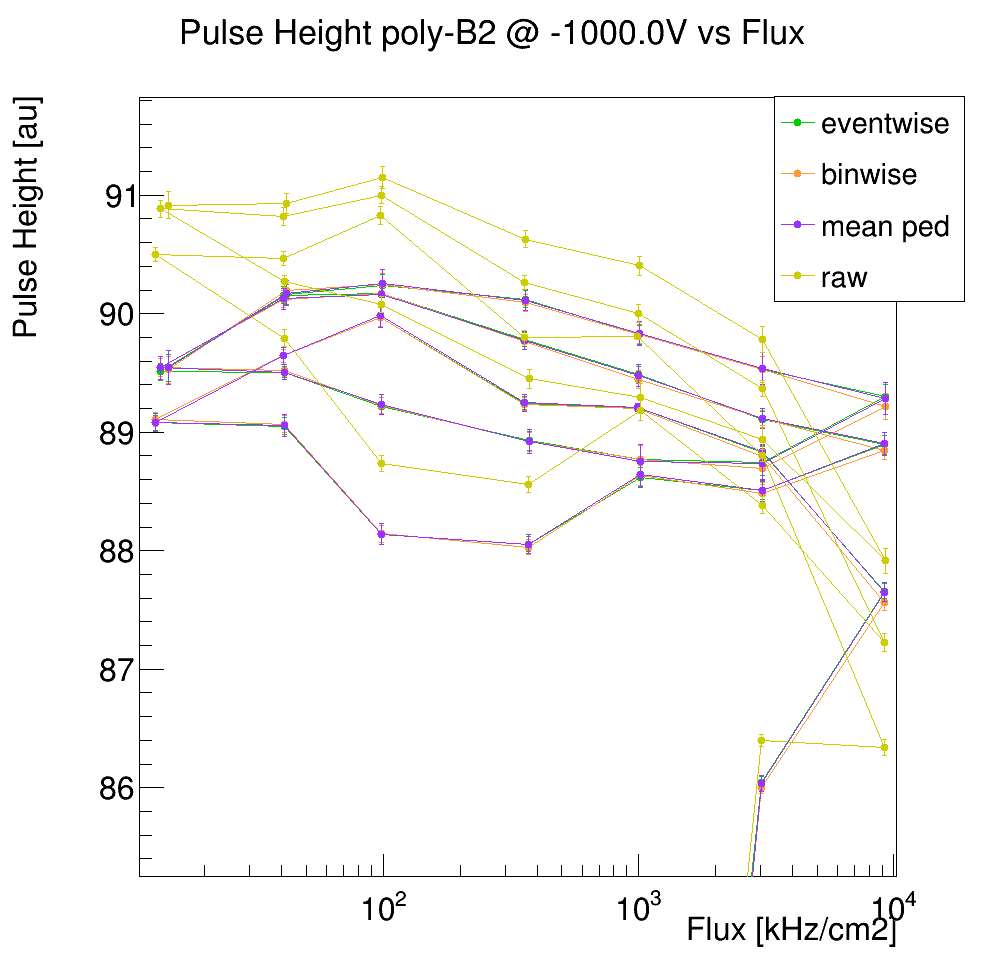
\includegraphics[width=7cm]{Pics/B2full}
	\end{center}
\end{frame}
% new frame ============================
\begin{frame}
	\frametitle{Signal B2}
	\begin{center}
		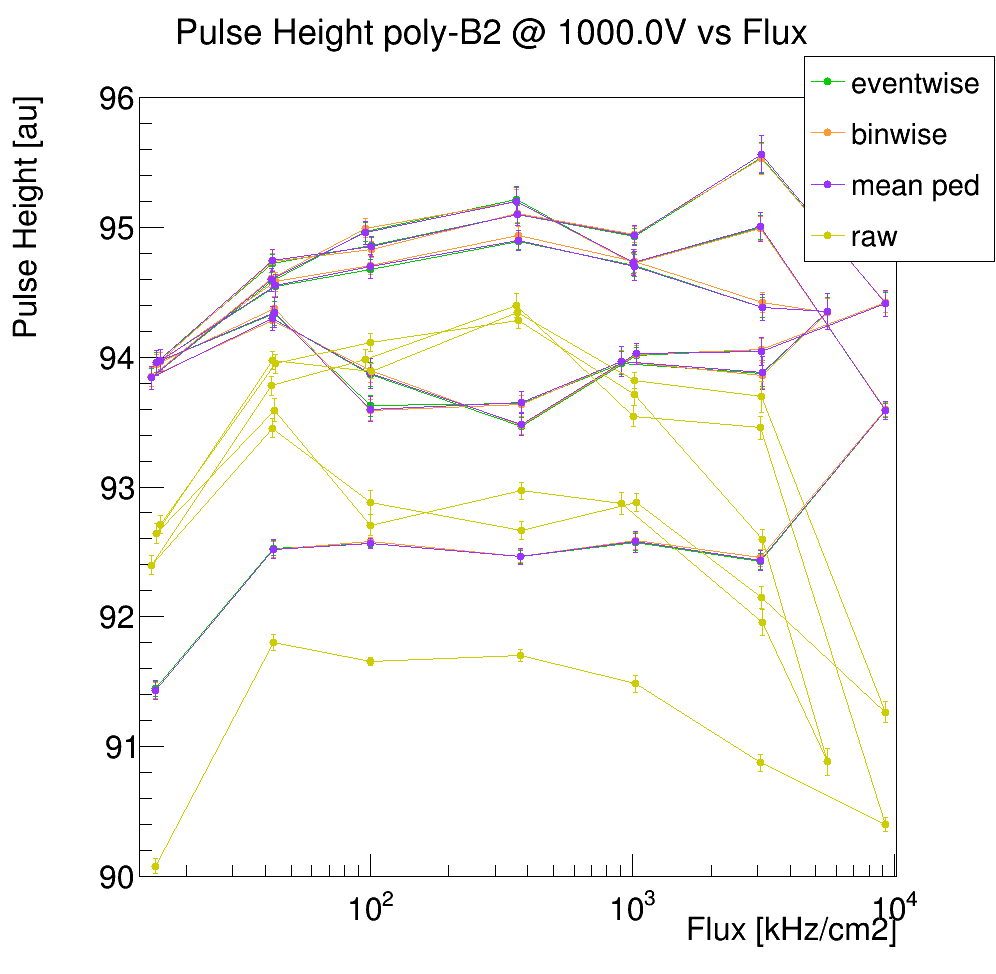
\includegraphics[width=7cm]{Pics/B2fullpos}
	\end{center}
\end{frame}
% new frame ============================
\begin{frame}
	\frametitle{Signal Poly-D}
	\begin{center}
		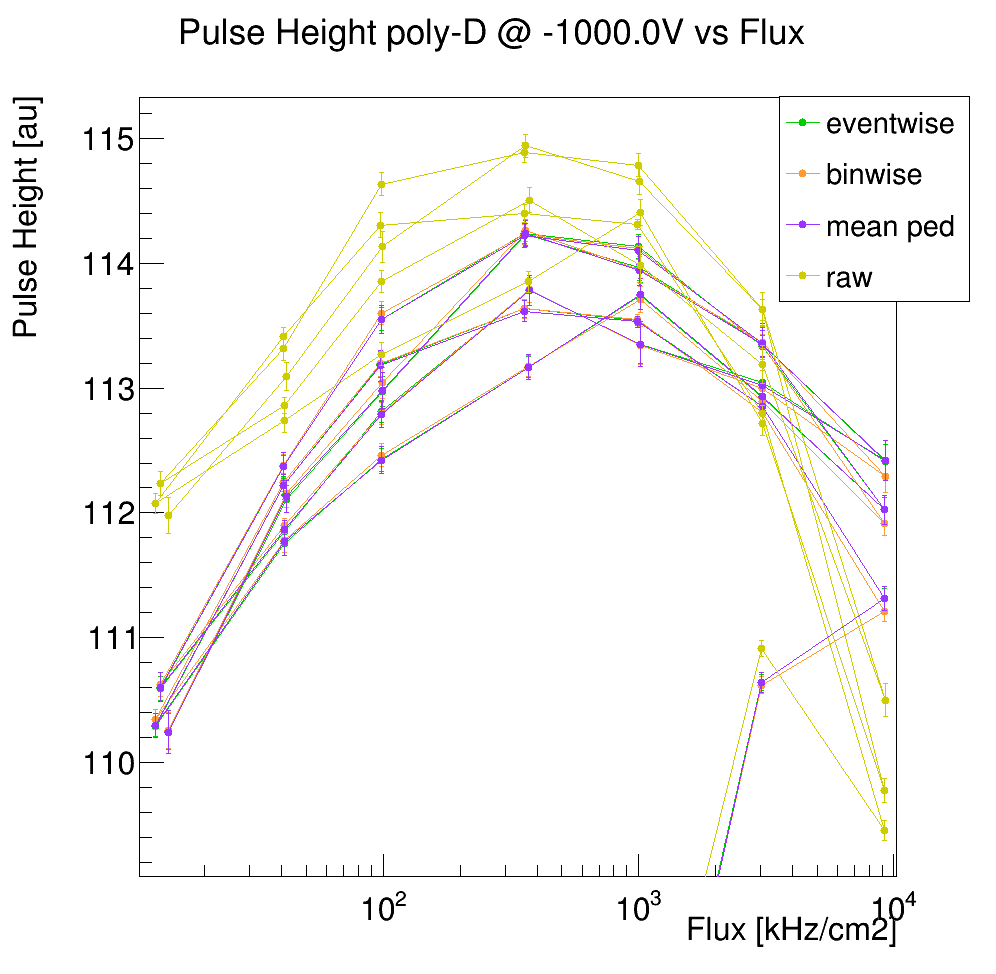
\includegraphics[width=7cm]{Pics/Dfullneg}
	\end{center}
\end{frame}
% new frame ============================
\begin{frame}
	\frametitle{Signal Poly-D}
	\begin{center}
		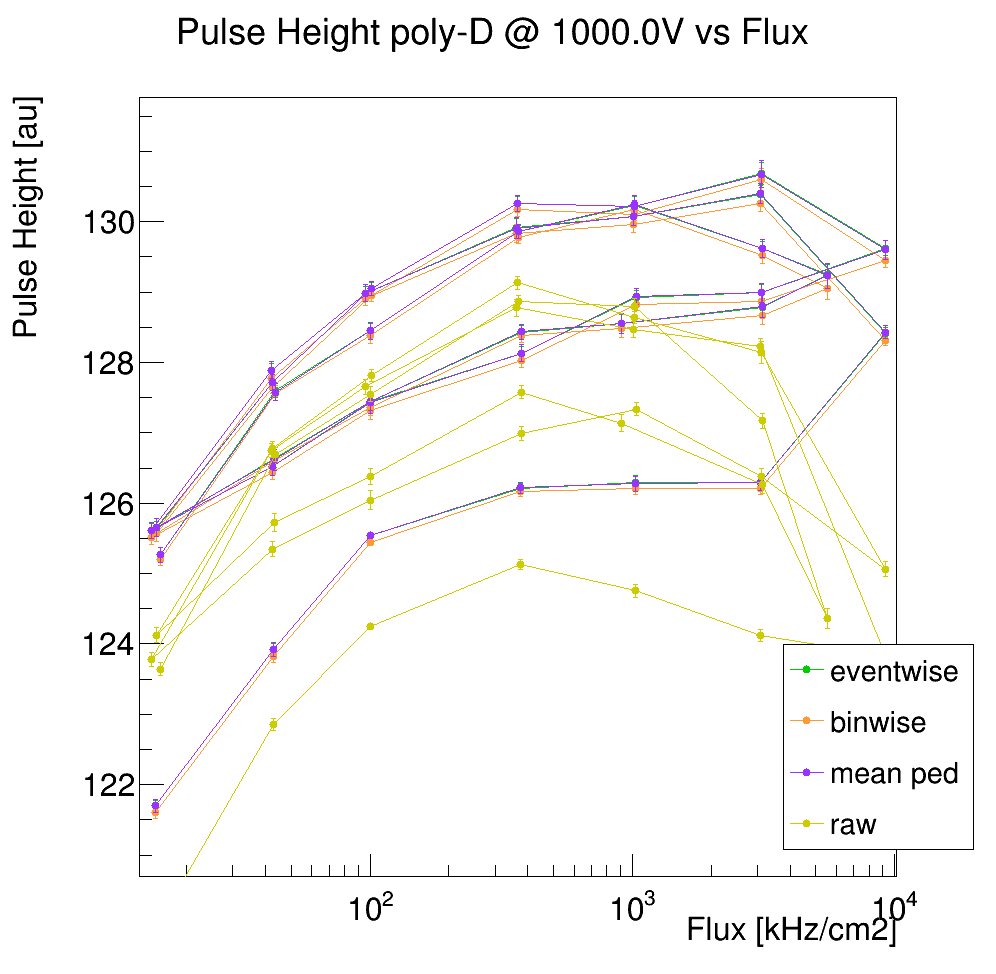
\includegraphics[width=7cm]{Pics/Dfullpos}
	\end{center}
\end{frame}
% ============================
% DOCUMENT END
\end{document}

